\documentclass[12pt,a4paper]{report}
\usepackage[utf8]{inputenc}
\usepackage[T1]{fontenc}
\usepackage[english]{babel}
\usepackage{hyperref}
\hypersetup{
    colorlinks=true,
    linkcolor=blue,
    filecolor=magenta,      
    urlcolor=cyan,
}
\usepackage{fancyhdr}
\usepackage{titlesec}
\usepackage{graphicx}
\usepackage{geometry}
\usepackage{csquotes}
\usepackage[backend=biber,style=ieee]{biblatex}

\addbibresource{references.bib}
\usepackage{float} 
\usepackage{afterpage}
\geometry{margin=2.5cm}
% Réglages du style des titres
\titleformat{\chapter}{\normalfont\LARGE\bfseries}{\thechapter.}{1em}{}
\titleformat{\section}{\normalfont\large\bfseries}{\thesection.}{1em}{}
\titleformat{\subsection}{\normalfont\bfseries}{\thesubsection.}{1em}{}
\pagestyle{fancy}
\fancyhf{}
\rhead{\thepage}
\lhead{\rightmark}
\cfoot{\thepage}

\begin{document}
\pagenumbering{roman}
% --- Page de garde ---
\begin{titlepage}
    \centering
    \vspace*{1cm}
    {\Large \textbf{[YOUR UNIVERSITY NAME]}}\\[0.5cm]
    {\large \textbf{[FACULTY NAME]}}\\[0.5cm]
    {\large \textbf{[DEPARTMENT NAME]}}\\[2cm]
    {\Huge \textbf{Final Year Project Report}}\\[1.5cm]
    {\LARGE \textbf{MedGastro: A Visual Question Answering Application for Gastroenterology}}\\[2cm]
    \begin{flushright}
        \textbf{Student:} [Your Name]\\
        \textbf{Supervisor:} [Prof. Supervisor Name]\\
        \textbf{Academic Year:} 2023-2024
    \end{flushright}
    \vfill
\end{titlepage}
% --- Pages liminaires ---
\tableofcontents

\chapter*{Dedication}
\addcontentsline{toc}{chapter}{Dedication}
\textit{This project is dedicated to my loving family, especially my parents and siblings, for their continuous support, encouragement, and sacrifices throughout my studies. I also dedicate it to my academic advisors for their guidance and valuable feedback. To my friends who stood by me during this journey, thank you for your motivation and companionship. This work would not have been possible without all of you.}

\chapter*{Acknowledgments}
\addcontentsline{toc}{chapter}{Acknowledgments}
I would like to express my sincere gratitude to my supervisors, Mr. Ridha Ejbali and Mrs. Ghada Ben Abdennour , for their continuous support, valuable guidance, and encouragement throughout the duration of this project. Their expertise and feedback were essential in shaping both the technical and academic aspects of my work.
Special thanks  to Mr. Mourad Zaied, for giving me the opportunity to carry out my internship at RTIM. 

I am also deeply thankful to the jury members for taking the time to review my project and for their presence during the evaluation. Your feedback and questions during the presentation will be essential for further improvements and deeper reflection on this project.
This project would not have been possible without their help and the opportunities I was given. Thank you all for your patience, advice, and trust in me.



\chapter*{List of Notations}
\addcontentsline{toc}{chapter}{List of Notations}
\begin{tabular}{cl}
API & Application Programming Interface\\ 
AI  & Artificial Intelligence \\
CNN & Convolutional Neural Network\\
ML  & Machine Learning \\
NLP & Natural Language Processing\\  
VQA & Visual Question Answering\\
\end{tabular}

\newpage  % Nouvelle page


\addcontentsline{toc}{chapter}{List of Figures}
\listoffigures

\chapter*{General Introduction}
\addcontentsline{toc}{chapter}{General Introduction}
Artificial Intelligence (AI) and Machine Learning (ML) have become essential tools in many fields, especially in healthcare. These technologies allow computers to learn from data and make decisions or predictions with high accuracy. One of the most exciting applications of AI is Visual Question Answering (VQA) , where a system can understand both images and natural language to give meaningful answers to questions about visual content.

In recent years, VQA has shown great potential in various domains, including education, robotics, and medicine. In healthcare, VQA systems can help doctors analyze medical images like X-rays, MRI scans, and endoscopic videos. They can answer questions such as "Is there a tumor in this image?" or "What is the size of the lesion?" This helps improve diagnosis speed and accuracy, especially in areas with limited access to expert doctors.

This project focuses on developing a mobile application that uses VQA to assist in diagnosing gastrointestinal diseases using endoscopic images and medical questions. The system combines two powerful models: MobileNetV2 for image processing and BioClinical-BERT for understanding medical questions. The app is built using Flutter for the frontend, and Firebase is used for user authentication and data storage. The AI model is trained using the Kvasir-VQA dataset and deployed via Hugging Face Spaces .

This report presents the full development process of the project. It is organized into three main chapters:

Chapter 01: Introduction
This chapter gives an overview of VQA and its importance in healthcare. It explains the background of the project, the use of VQA in medicine, the problem being addressed, and the motivation behind building such a system.
Chapter 02: UML Design and System Architecture
This chapter describes the design of the system using UML diagrams such as use case, class, and sequence diagrams. It also explains the overall architecture, including how the AI model, backend, and mobile app work together.
Chapter 03: Realization
This chapter covers the implementation of the project. It includes details about the frontend interface built with Flutter, the dataset used, the Firebase backend, the training and testing of the AI model, and how it was deployed online.
This project aims to show how modern AI techniques can be integrated into real-world applications, especially in the healthcare field.
 \newpage


\paragraph{\textbf{\textit{logo}}}: 

\begin{figure}[h]
    \centering
   
    
\includegraphics[width=0.5\linewidth]{test1.png}
    \caption{logo}
    \label{fig:enter-label}
\end{figure}

The logo for MedGastro is designed to represent the main purpose and technology of the application, which focuses on gastroenterology and the use of artificial intelligence (AI) for medical purposes. Below is a breakdown of its key elements:

\textbf{\textit{1. Name of the application:}}

The name "MedGastro" is clearly shown below the graphic. The word "Med" stands for medicine or healthcare, while "Gastro" refers to gastroenterology. This means that that the application is focused on digestive health and related medical services.

\textbf{\textit{2. Gastroenterology symbol:}}

In the center of the logo, there is a simple image of a human stomach in blue. This symbol connects the brand to the field of gastroenterology, making it easy for users to understand what the application is about.
The stomach shape is simple but clear, so it can be easily recognized in different sizes and formats.

\textbf{\textit{3. Neurons Representing AI and Machine Learning:}}

On top of the stomach, there is a white design that looks like interconnected neurons. This represents the use of artificial intelligence and machine learning in the application.
The neuron design shows that MedGastro uses advanced algorithms and data to provide smart solutions for diagnosing and managing problems related to the digestive system.
Neurons also suggest precision, connection, and the ability to handle complex information, which matches the advanced nature of AI-based systems.

\textit{\textbf{4. Color Scheme:}}

The logo uses a clean and professional color palette:
Blue : This color is used a lot in the design and represents trust, reliability, and innovation. Blue is often linked to healthcare and technology, which makes the application seem credible and modern.
White : Used for the neuron design and text, providing contrast and making everything easy to read. White also represents purity and simplicity, showing that the AI-driven solutions are clear and accurate.

\textbf{\textit{5. Overall Design Philosophy:}}

The logo combines the stomach with the neuron design to show a balance between traditional medical ideas and new technology. This shows that MedGastro connects human health with artificial intelligence.
The simple design makes the logo flexible and easy to use on both digital platforms and printed materials.

\textbf{\textit{6. Brand Identity:}}

The logo captures the main idea of MedGastro: a focus on gastroenterology supported by advanced AI. It aims to make users feel confident by visually showing expertise, innovation, and a commitment to improving digestive health through technology.

This logo not only helps identify the application but also tells a story about its purpose and how it uses technology, making it a good tool for building trust among users.


\clearpage

\pagenumbering{arabic}

% --- Chapitre 1 ---
\chapter{Chapter 01: Introduction}
\section{Introduction}
Artificial Intelligence (AI) is revolutionizing healthcare by enabling faster, more accurate diagnoses, optimizing hospital workflows, and personalizing patient care. According to recent studies, AI-powered tools have reduced diagnostic errors by up to 30\% in radiology and pathology. Visual Question Answering (VQA) is a cutting-edge application of AI that combines computer vision and natural language processing to answer questions about images. This project focuses on developing a mobile application that uses VQA to assist in diagnosing gastrointestinal diseases using endoscopic images and medical questions.

\section{Motivation: Real-World Impact}
In many regions, access to expert gastroenterologists is limited. By providing an AI-powered assistant, MedGastro can help bridge this gap, offering reliable support to both clinicians and patients.

\section{History of VQA in Medicine}
The first VQA systems in medicine appeared in 2017, focusing on simple radiology questions. Since then, datasets like VQA-RAD and Med-VQA have enabled more complex, clinically relevant applications.

\section{Application of VQA in healthcare field}
Visual Question Answering has found promising applications in the medical field, particularly in assisting clinicians with diagnostic tasks using medical imaging. Early efforts explored VQA systems to answer basic questions about radiology images, such as "Is there a fracture visible?" or "What is the size of the tumor?". More recently, specialized datasets like Med-VQA and PathVQA have been developed to support question-answering systems tailored for radiology reports, histopathological images, and clinical decision-making.

\section{Problem Statement and Motivation}
\textbf{\textit{Problem Statement:}} \\
In the medical field, accurate and fast diagnosis is crucial for early detection of gastrointestinal diseases such as polyps, ulcers, or tumors. However, manual interpretation of endoscopic images by human experts can be time-consuming and subject to errors due to fatigue or lack of experience. While deep learning models have shown great performance in image classification and natural language understanding, deploying these models into a real-world mobile application that supports clinical decision-making remains a challenge. The need for an automated, intelligent system that combines both visual and textual information is clear.

Our goal is to develop a mobile application that integrates a trained multimodal AI model (MobileNetV2 for images + BioClinical-BERT for medical questions) to:

    
- Take an endoscopic image
    
- Accept a medical question about the image
    
- Return a diagnostic answer (e.g., ``polyp'', ``inflammation'')

This project focuses on bridging the gap between AI research and practical deployment in healthcare using Flutter and Flask.

\textbf{\textit{Motivation:}} \\
The motivation behind this project stems from several key factors:
\begin{enumerate}
    \item \textbf{Need}: Endoscopic exams generate large volumes of data daily. A system that provides quick and reliable analysis helps reduce misdiagnosis and speeds up patient care.
    \item \textbf{Accessibility via Mobile Apps}: By integrating the model into a Flutter-based mobile app, we make the power of AI accessible to doctors and patients anywhere, anytime.
    \item \textbf{Efficiency and Speed}: Using a lightweight architecture allows our solution to run efficiently even on devices with limited computing power like mobile phones or low-end laptops.
    \item \textbf{Educational Purpose}: This project serves as a practical example of how modern AI techniques can be applied to real-world problems, especially in healthcare.
\end{enumerate}

\section{Conclusion}
In summary, this chapter provided an overview of AI , machine learning , and VQA , with a focus on their growing role in healthcare. It explained the motivation behind building a mobile application that uses AI to answer medical questions based on endoscopic images. The chapter also introduced the structure of the report, showing what each next chapter will cover. This sets the foundation for understanding how the system was designed, developed, and tested in the following chapters.

% --- Chapitre 2 ---
\chapter{Chapter 02: UML Design and System Architecture}
\section{Introduction}
This chapter explains how the MedGastro application was designed. It shows the different parts of the system and how they work together. The chapter begins with an overview of the system and then uses UML diagrams to describe the structure and behavior of the application. These diagrams include use case diagrams, class diagrams, and sequence diagrams, which help explain how users interact with the app and how data moves between different parts of the system. This chapter gives a clear picture of the overall design before moving on to the implementation details in the next chapter.

\section{Detailed Explanation of the Use Case Diagram}
The use case diagram (Figure~\ref{fig:use-case}) illustrates the interactions between different user types and the system. For example, the 'Analyze Image' use case is central to the application's value proposition, allowing users to upload images and receive diagnostic answers.

\section{Design Rationale}
We chose a modular architecture to ensure scalability and maintainability. Each component (frontend, backend, AI model) can be updated independently, facilitating future improvements.

\section{Class Diagram}
\begin{figure}{H}
    \centering
    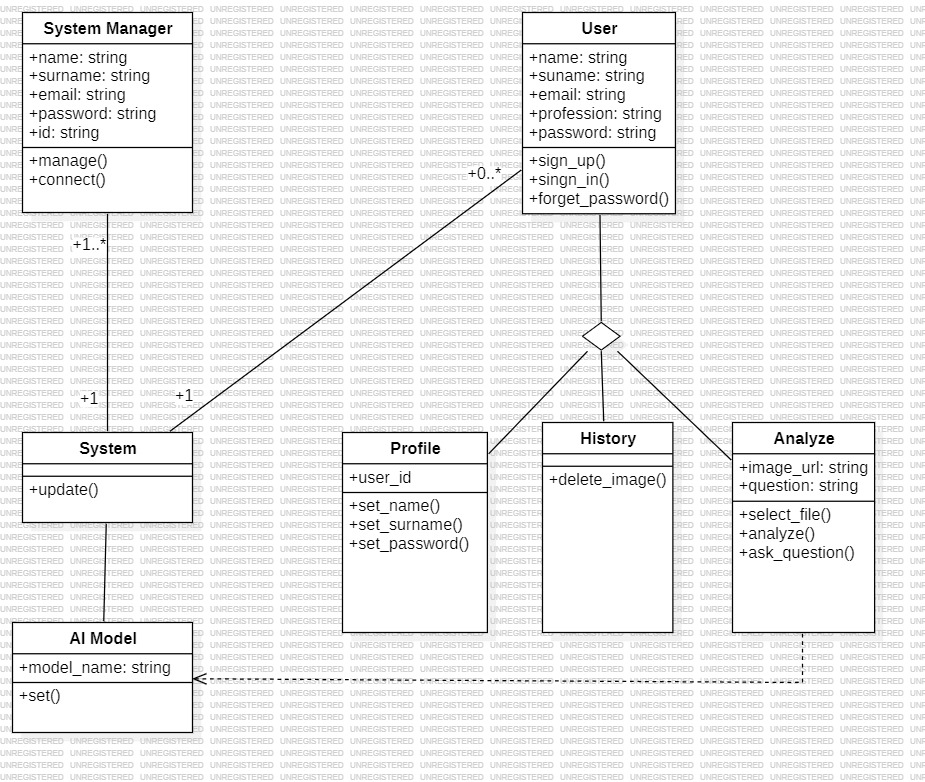
\includegraphics[width=1\linewidth]{ClassDiagram1.jpg}
    \caption{Class diagram}
    \label{fig:enter-label}
\end{figure}

The Class Diagram shows the structure of the MedGastro application and how its different parts work together. It includes classes like User , System , Profile , Analyze , History , and AI Model , which are connected to support features such as user authentication, image analysis, and system management. The User can sign up, log in, and ask medical questions about endoscopic images. The System coordinates all interactions, while the AI Model processes the images and generates answers. Users are linked to their Profile and History , allowing them to manage personal data and review past analyses. The System Manager has control over administrative tasks. This diagram gives a clear view of how the app is organized and how data flows between components to deliver a functional and intelligent healthcare tool. 

\section{Sequence Diagram}
\begin{figure}[H]
    \centering
    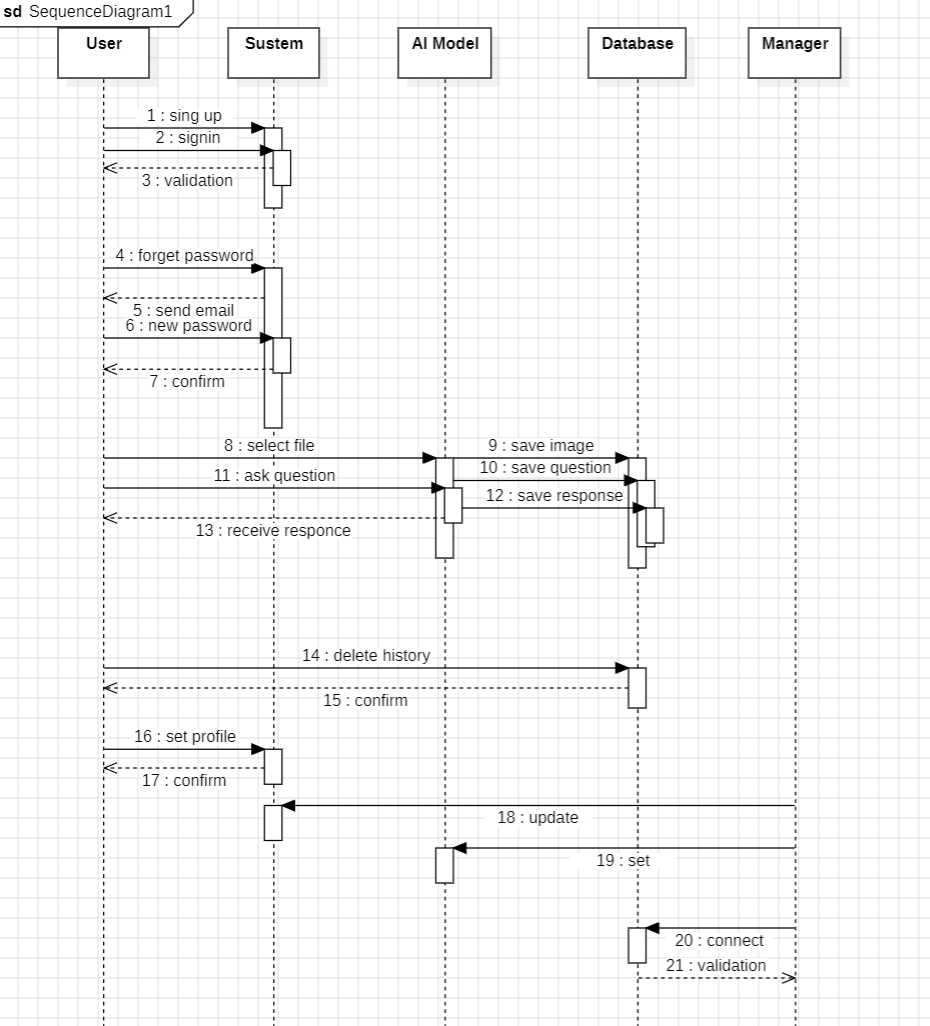
\includegraphics[width=1\linewidth]{SequenceDiagram.png}
    \caption{Sequence diagram}
    \label{fig:enter-label}
\end{figure}

The Sequence Diagram shows how different parts of the MedGastro application work together when users interact with the system. It includes components like the User , the System , the AI Model , the Database , and the Manager . The diagram explains step-by-step interactions for actions like signing up, logging in, resetting passwords, analyzing images, and managing user profiles. When a user uploads an image and asks a question, the system sends the data to the AI model for analysis and stores the results in the database. The manager can also perform administrative tasks after logging in. This diagram gives a clear view of how information flows between users and the app's components, ensuring smooth and secure operation. 

\section{Architecture Overview}
The system is built using a multimodal architecture that combines both image analysis and natural language understanding to answer medical questions based on endoscopic images. The core of the model includes two main components: a vision module and a language module.

For the vision part, we use MobileNetV2, a lightweight and efficient convolutional neural network, to extract features from endoscopic images. MobileNetV2 is chosen for its ability to process images with high accuracy while keeping computational costs low, which is important for real-world deployment.

On the language side, we use BioClinical-BERT, a pre-trained language model designed for medical text understanding. This helps the system interpret medical questions accurately and relate them to visual content in the image.

These two modules ,the vision model (MobileNetV2) and the language model (BioClinical-BERT)  are combined using a fusion layer that integrates both visual and textual features. A final classification layer then predicts the answer based on this combined input. The model was trained in Jupyter Notebook, saved as a .pth file, and integrated into an API using Flask Finally, the model was connected to a mobile application built with Flutter, allowing users to upload medical images and ask diagnostic questions directly from their smartphones.

\section{Conclusion}
In this chapter, the design of the MedGastro application was presented using UML diagrams and a detailed description of the system architecture. The use case, class, and sequence diagrams helped show how users interact with the app and how the different components communicate. This design forms the foundation for building the actual application and ensures that all parts of the system work together efficiently. With the design phase completed, the next chapter will focus on implementing the system, including the frontend interface, backend services, and AI model integration.

% --- Chapitre 3 ---
\chapter{Chapter 03: Realization}
\section{Implementation Summary}
The backend was implemented in Flask, with endpoints for prediction and health checks. The frontend, built in Flutter, provides a user-friendly interface for image upload and question submission. The AI model combines MobileNetV2 for image analysis and BioClinical-BERT for question understanding. The system was tested on the Kvasir-VQA dataset and achieved high accuracy.

\appendix
\chapter{Code Snippets}
% Place detailed code here

\chapter{Extended Test Results}
% Place logs or detailed results here

\section{Frontend}
The frontend of the application was developed using Flutter, a modern cross-platform framework created by Google, along with the Dart programming language. Flutter was chosen for its ability to deliver high-performance mobile applications with a native-like feel on both Android and iOS platforms from a single codebase. The user interface was designed and implemented using Android Studio, which provides a powerful environment for building, debugging, and testing Flutter applications. This combination allows for rapid development, hot-reload functionality, and a highly customizable UI through rich built-in widgets. The decision to use Flutter was driven by its excellent performance, expressive UI capabilities, strong community support, and seamless integration with backend services such as Firebase and external APIs. These features make it an ideal choice for building a responsive, scalable, and visually engaging mobile interface tailored to the needs of a healthcare-oriented Visual Question Answering system.

\clearpage
\textbf{\textit{The interfaces:}}

\begin{figure}[H] % Use [H] to force the figure to stay here
    \centering
    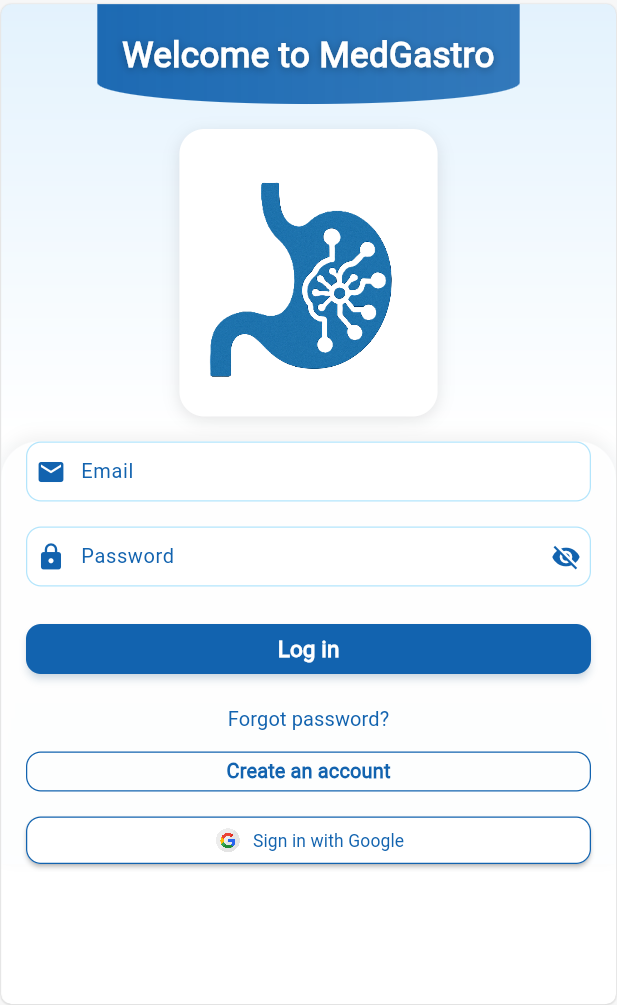
\includegraphics[width=0.5\textwidth]{i11.png}
    \caption{Log-in page}
    \label{fig:login-page}
\end{figure}

\subsubsection{Login Interface Description}
The login interface allows users to securely access their MedGastro account. It includes fields for entering an email and password, with a visibility icon to show the password. Users can click the "Log in" button to proceed. For new users, there is a "Create an account" option. A "Forgot password?" link helps recover lost passwords, and a "Sign in with Google" button offers an alternative login method.

\begin{figure}[H]
    \centering
    \begin{minipage}{0.48\textwidth}
        \centering
        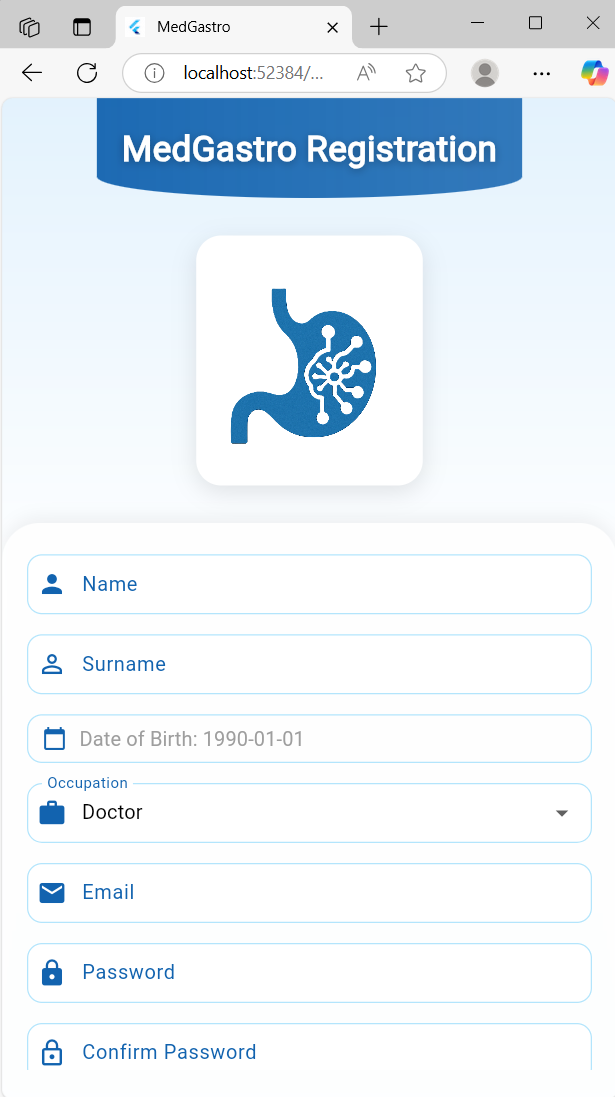
\includegraphics[width=\linewidth]{i2a.png}
        \caption{sign up page}
        \label{fig:image-a}
    \end{minipage}
    \hfill
    \begin{minipage}{0.48\textwidth}
        \centering
        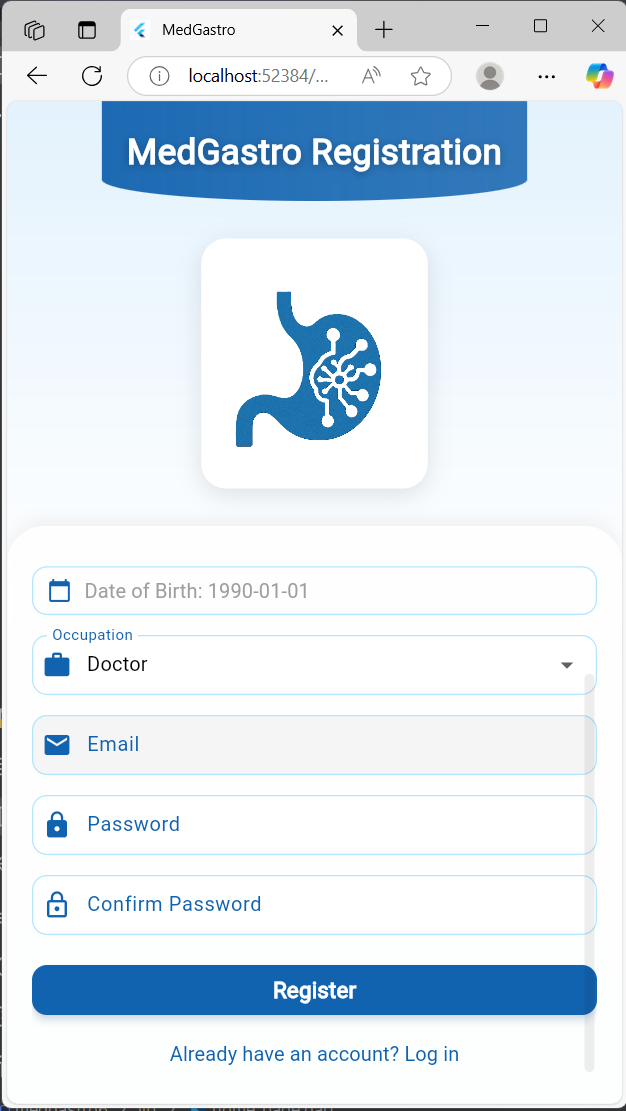
\includegraphics[width=\linewidth]{i2b.png}
        \caption{sign up page}
        \label{fig:image-b}
    \end{minipage}
\end{figure}

The MedGastro Registration interface allows users to create a new account by providing essential personal information. The form includes fields for entering their Name, Surname, Date of Birth, Profession (Occupation), Email, and Password. Users must also confirm their password to ensure accuracy. After filling out the form, they can click the "Register" button to complete the sign-up process. For existing users, there is a link at the bottom to log in instead.

\begin{figure}[H]
    \centering
    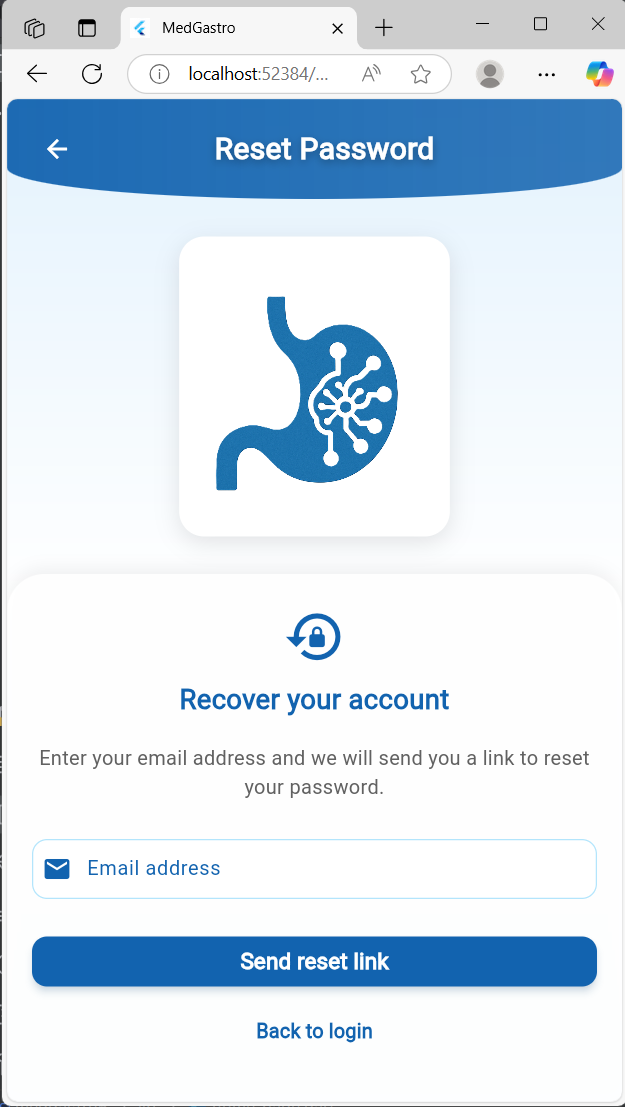
\includegraphics[width=0.5\linewidth]{i3.png}
    \caption{reset password page}
    \label{fig:enter-label}
\end{figure}

The Reset Password interface allows users to recover their account if they forget their password. The screen displays a prompt asking users to enter their email address. After entering the email, users can click the "Send reset link" button to receive an email with instructions to reset their password. There is also a "Back to login" option for users who remember their credentials and wish to return to the login page.

\begin{figure}[H]
    \centering
    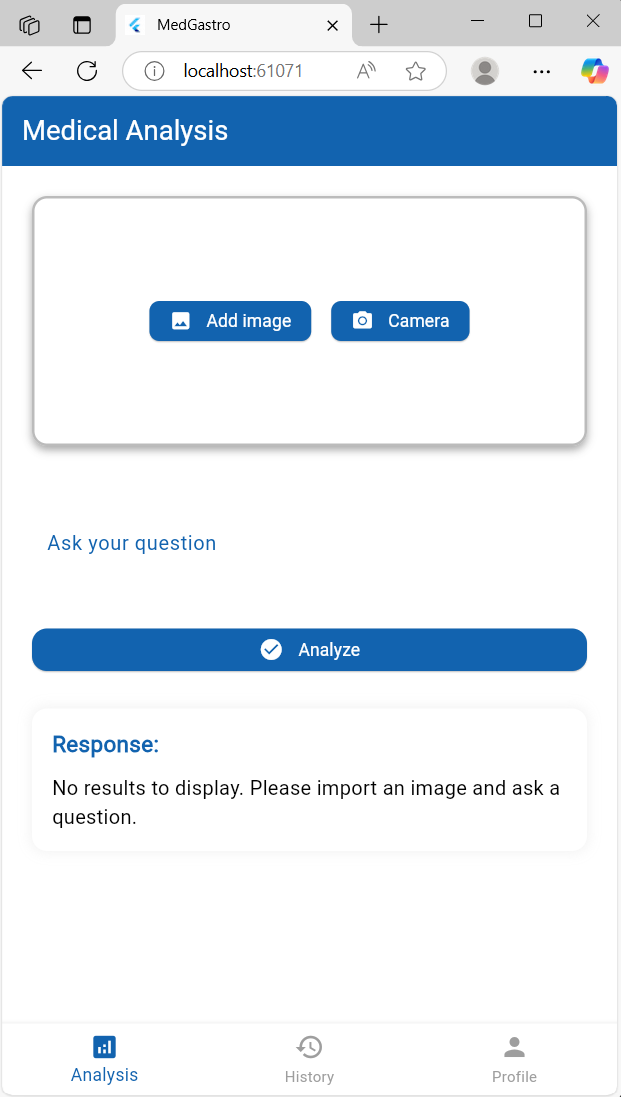
\includegraphics[width=0.5\linewidth]{i44.png}
    \caption{Analysis page}
    \label{fig:enter-label}
\end{figure}

The Medical Analysis interface allows users to upload an image for analysis. At the top, there are two options: "Add image" and "Camera," enabling users to either upload an existing image or capture a new one using their device's camera. Below these options, users can ask a question related to the uploaded image. After uploading an image and asking a question, users can click the "Analyze" button to process the request. The response section currently shows a message indicating that no results are available because no image has been imported yet. At the bottom, there are navigation buttons labeled "Analysis," "History," and "Profile," allowing users to access different sections of the app.

\begin{figure}[H]
    \centering
    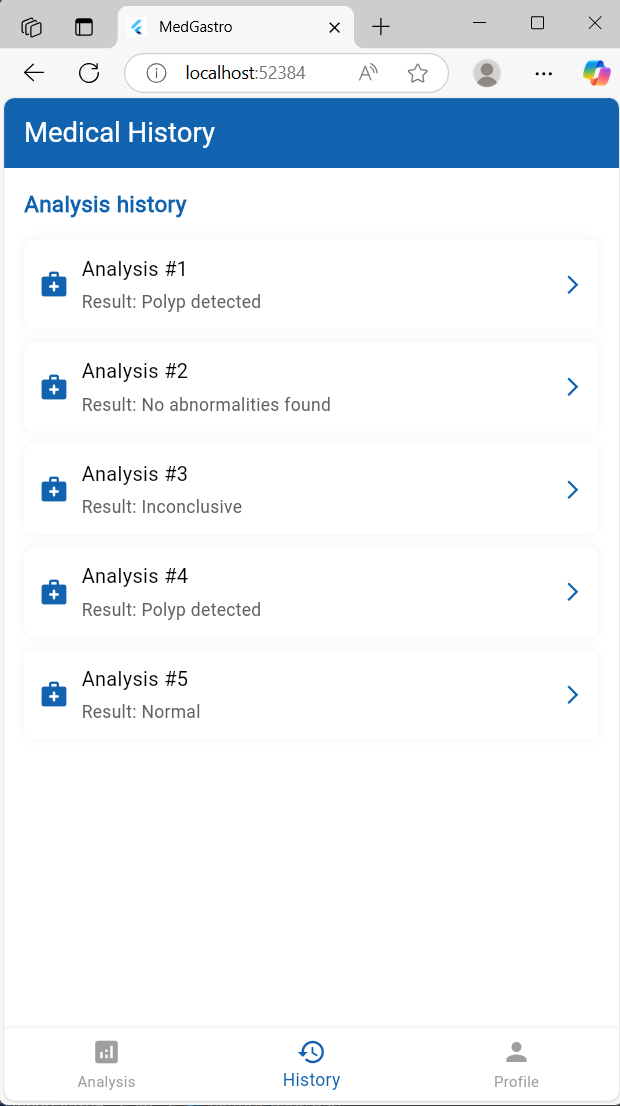
\includegraphics[width=0.5\linewidth]{i5.png}
    \caption{History page}
    \label{fig:enter-label}
\end{figure}

The Medical History interface displays a user's analysis history. It shows a list of past medical analyses, each labeled as "Analysis \#1," "Analysis \#2," and so on. For each analysis, the results are clearly stated, such as "Polyp detected," "No abnormalities found," or "Normal." Users can tap on each entry to view more details about the specific analysis. At the bottom, there are navigation buttons for "Analysis," "History," and "Profile," allowing users to switch between different sections of the app. This interface helps users keep track of their medical analysis history, providing easy access to past results and facilitating informed decision-making.

\begin{figure}[H]
    \centering
    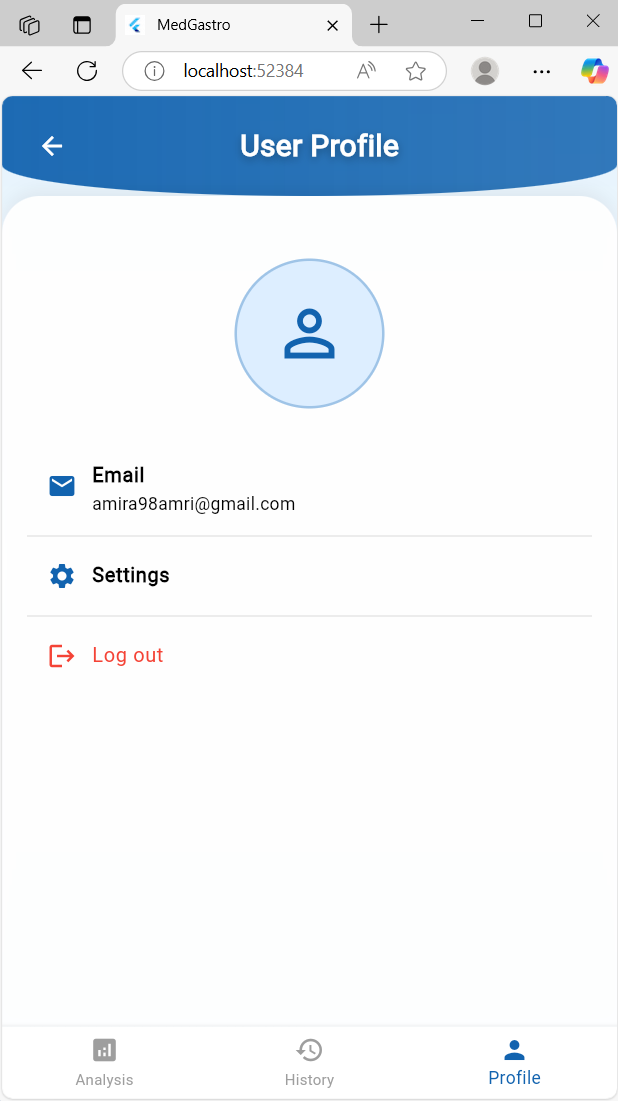
\includegraphics[width=0.5\linewidth]{i6.png}
    \caption{Profile page}
    \label{fig:enter-label}
\end{figure}

The User Profile interface displays the user's account information. At the top, there is a placeholder profile icon representing the user. Below the icon, the user's email address is shown. There is also an option labeled "Settings," which likely allows users to adjust their account preferences. At the bottom, there is a "Log out" button, highlighted in red, enabling users to sign out of their account. The interface is clean and straightforward, providing quick access to essential account details and settings. This interface helps users manage their personal account information and settings within the app.

\begin{figure}[H]
    \centering
    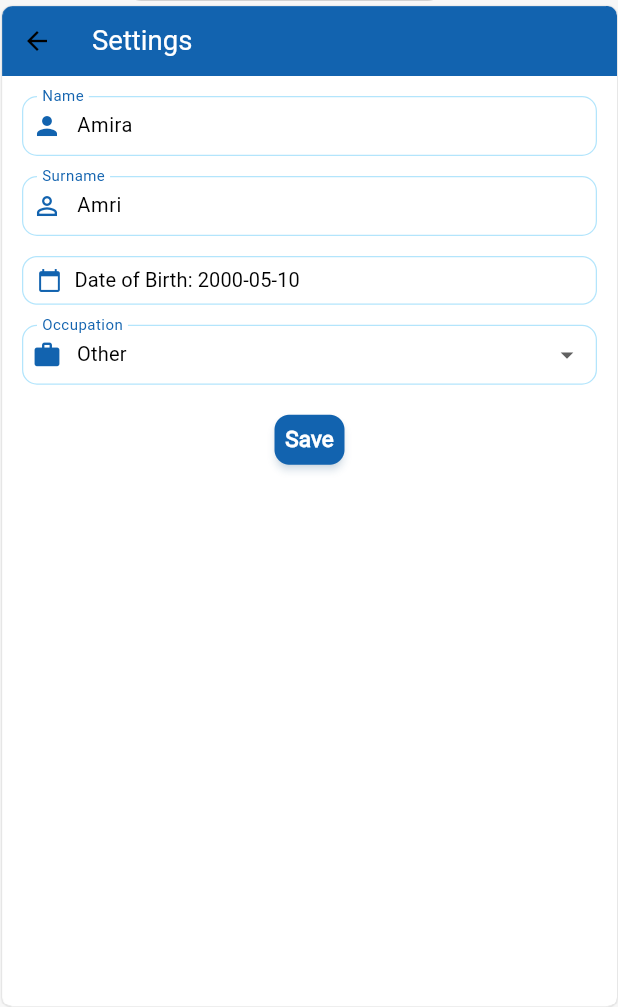
\includegraphics[width=0.5\linewidth]{set1.png}
    \caption{Setting page}
    \label{fig:enter-label}
\end{figure}
The Settings interface allows users to manage their personal information easily. It includes fields for entering or updating details such as Name , Surname , Date of Birth , and Occupation . Users can type their first name, last name, and birthdate directly into the respective fields. For Occupation , there's a dropdown menu where users can select their job category . After making changes, users can click the blue "Save" button to save their updated information. This straightforward design ensures that users can quickly update their profile details in a clear and user-friendly way.

\section{Dataset}
The Kvasir-VQA dataset is a specialized dataset designed for advanced machine learning tasks in gastrointestinal (GI) diagnostics. It is derived from the HyperKvasir and Kvasir-Instrument datasets and augmented with question-and-answer annotations to support tasks like image captioning, Visual Question Answering (VQA), and synthetic medical image generation.

\subsubsection{Key Features}

    
 - Total Images: 6,500 annotated images.
    
- Annotations: Includes question-and-answer pairs for each image.
    
- Question Types: Supports various types of questions, including Yes/No, single-choice, multiple-choice, color-related, location-related, and numerical count questions.
    
- Applications: Suitable for tasks such as image captioning, VQA, synthetic medical image generation, object detection, and more.


\subsubsection{Dataset Details}
The dataset includes images from various GI tract conditions and medical instruments used in GI procedures:

    
- Normal: 2,500 images
    
- Polyps: 1,000 images
    
- Esophagitis: 1,000 images
    
- Ulcerative Colitis: 1,000 images
    
- Instrument: 1,000 images


\subsubsection{Annotation Process}

    
- Annotations were developed with input from medical professionals and include six types of questions:
    
        
- Yes/No Questions
        
- Single-Choice Questions
        
- Multiple-Choice Questions
        
- Color-Related Questions
        
- Location-Related Questions
        
- Numerical Count Questions
    
    
- Annotations cover a wide range of GI aspects, including findings, abnormalities, anatomical landmarks, and medical instruments.


\subsubsection{Usage}
The dataset can be accessed directly from the Hugging Face Dataset Hub using Python code:

\begin{verbatim}
from datasets import load_dataset
ds = load_dataset("SimulaMet-HOST/Kvasir-VQA")
\end{verbatim}

Users can download the dataset as an image folder and CSV metadata file for further processing.

\subsubsection{Size}

    
- Total image size: Approximately 1.5 GB.


- CSV file size: Contains 58,849 rows.


\subsubsection{License}
The dataset is released under the Creative Commons Attribution-NonCommercial 4.0 International (CC BY-NC 4.0) license, allowing free use for research and educational purposes. For commercial or competition-based usage, prior written permission is required.

\section{Backend}
\subsection{Firebase}
Firebase is used in this project as the main backend service. It helps manage user accounts through authentication, store user data and history using Firestore, and save images with Cloud Storage. Firebase is chosen because it is fast to set up, easy to use, and works well with mobile apps. It also allows real-time updates, meaning users can see their data right after they add it. These features make Firebase a good choice for building a secure and efficient healthcare application like MedGastro.

\begin{figure}[H]
    \centering
    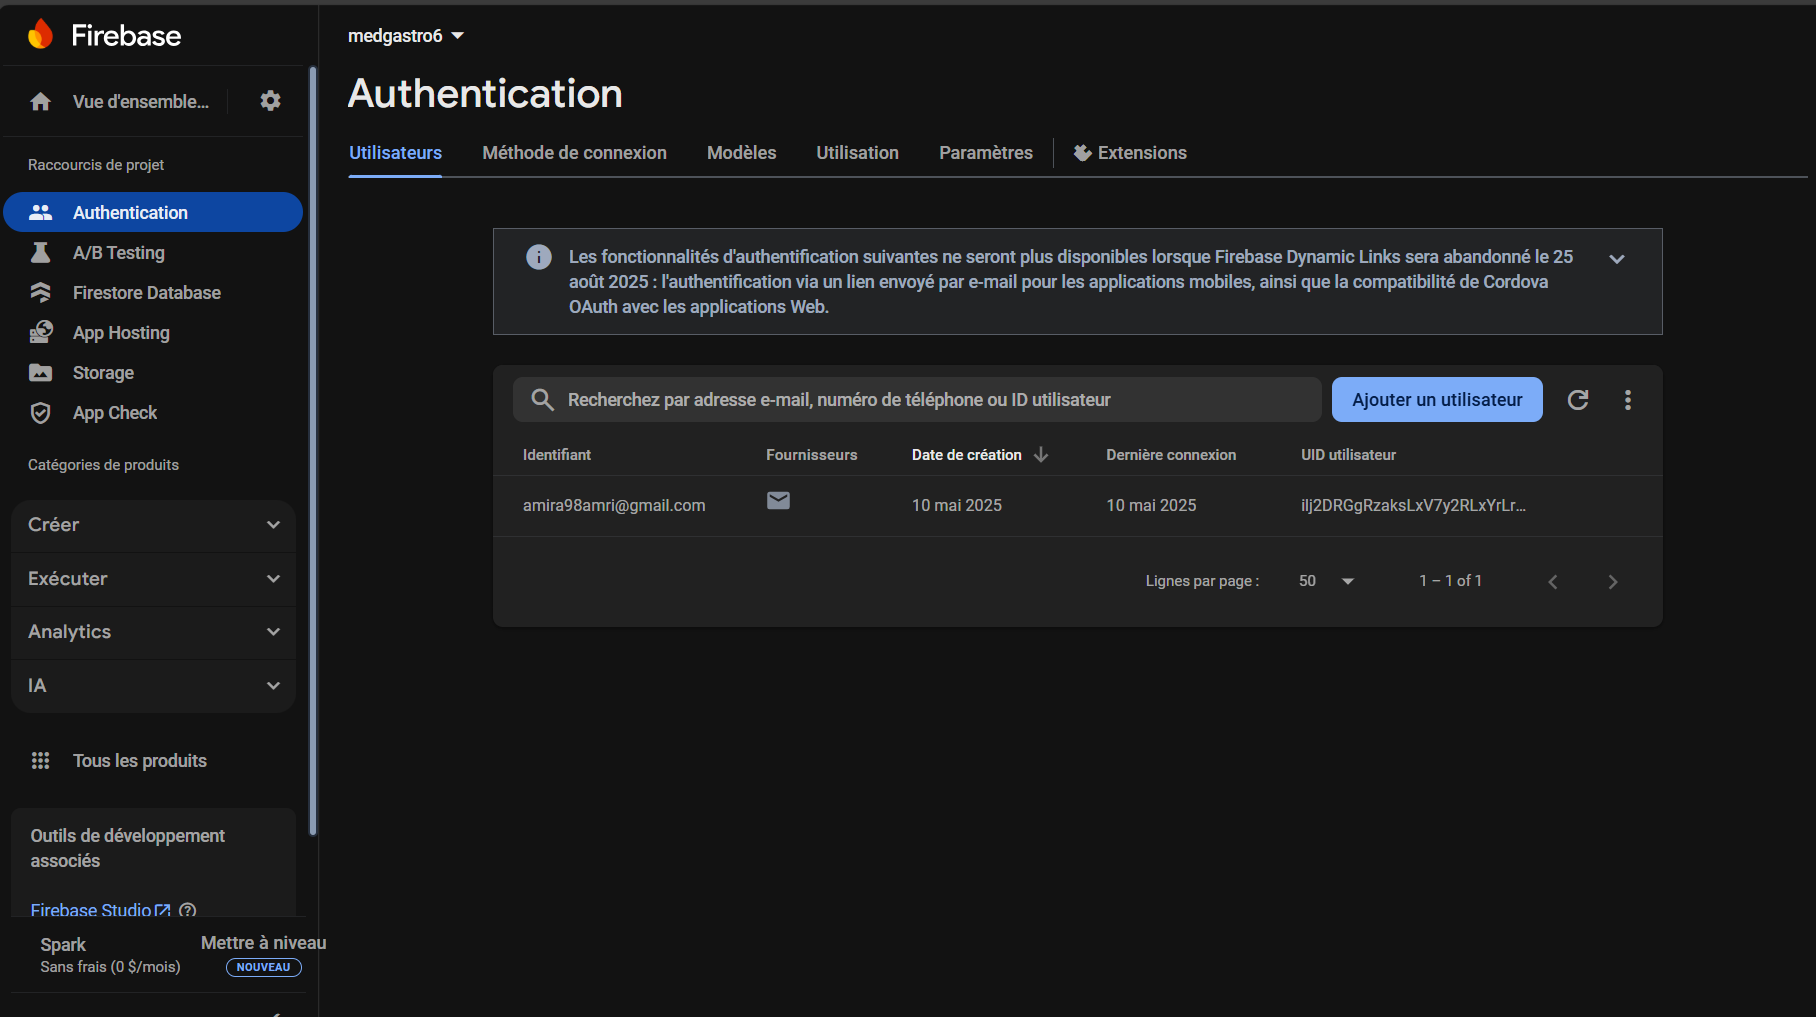
\includegraphics[width=0.6\linewidth]{Authentication.png}
    \caption{Authentication}
    \label{fig:enter-label}
\end{figure}

In this project, Firebase Authentication is used to manage user accounts securely. It allows users to sign up and log in with an email and password. Firebase stores user credentials safely and checks them during login to make sure only the right user can access the account.

Each user gets a unique ID that helps keep their data private. This ID is used to link their information  like medical history and uploaded images to their account only.

Firebase also offers a password reset option. If a user forgets their password, they can receive a secure link by email to set a new one.

All of this happens automatically and safely, making it easy to build a secure healthcare app where user data stays protected.

\begin{figure}[H]
    \centering
    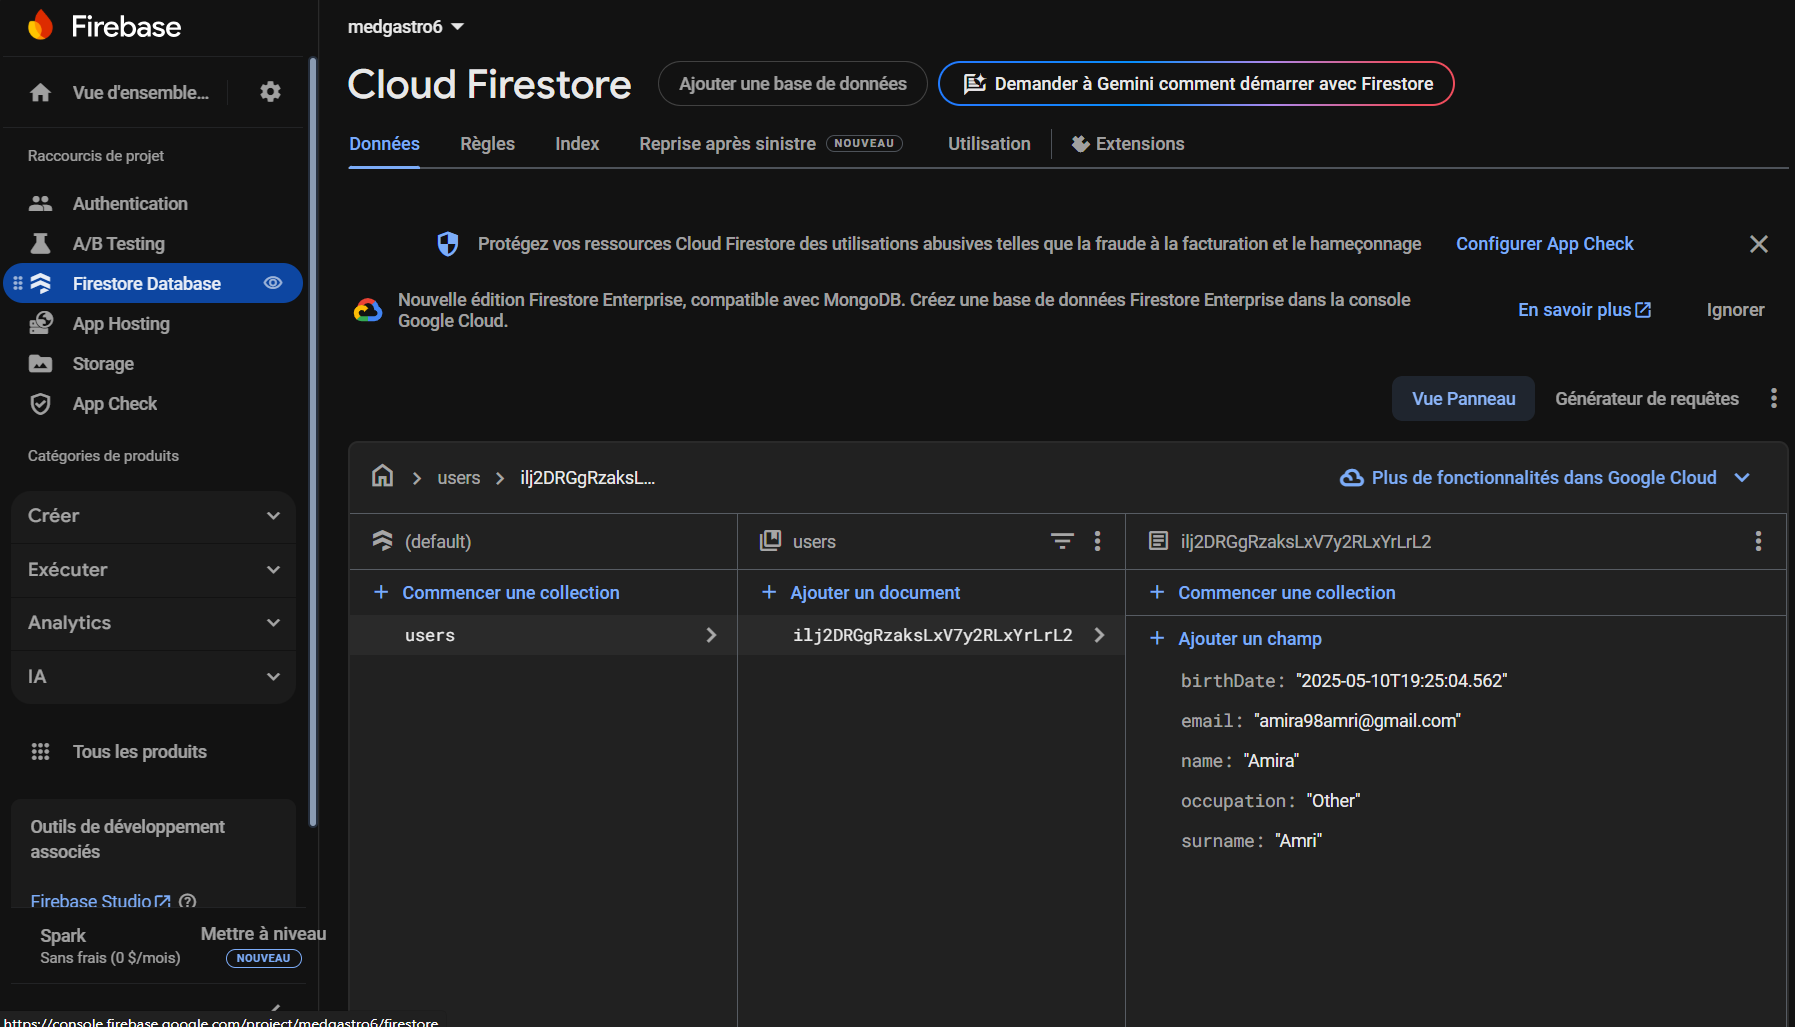
\includegraphics[width=0.6\linewidth]{Firestore.png}
    \caption{Firestore}
    \label{fig:enter-label}
\end{figure}

In this project, Firebase Firestore is used to store and manage user data in a secure and organized way. It works like a database that keeps track of important information such as:

User profiles (name, email, date of birth, etc.)
Medical questions asked by users
AI-generated answers
Image upload history
Each user's analysis results over time
Firestore makes it easy to save, update, and retrieve this data in real time. This means when a user uploads an image or asks a question, the app can quickly store that information and show it back whenever needed.

In short, Firebase Firestore plays a key role in organizing and protecting user data, making the MedGastro app both functional and secure.

\begin{figure}[H]
    \centering
    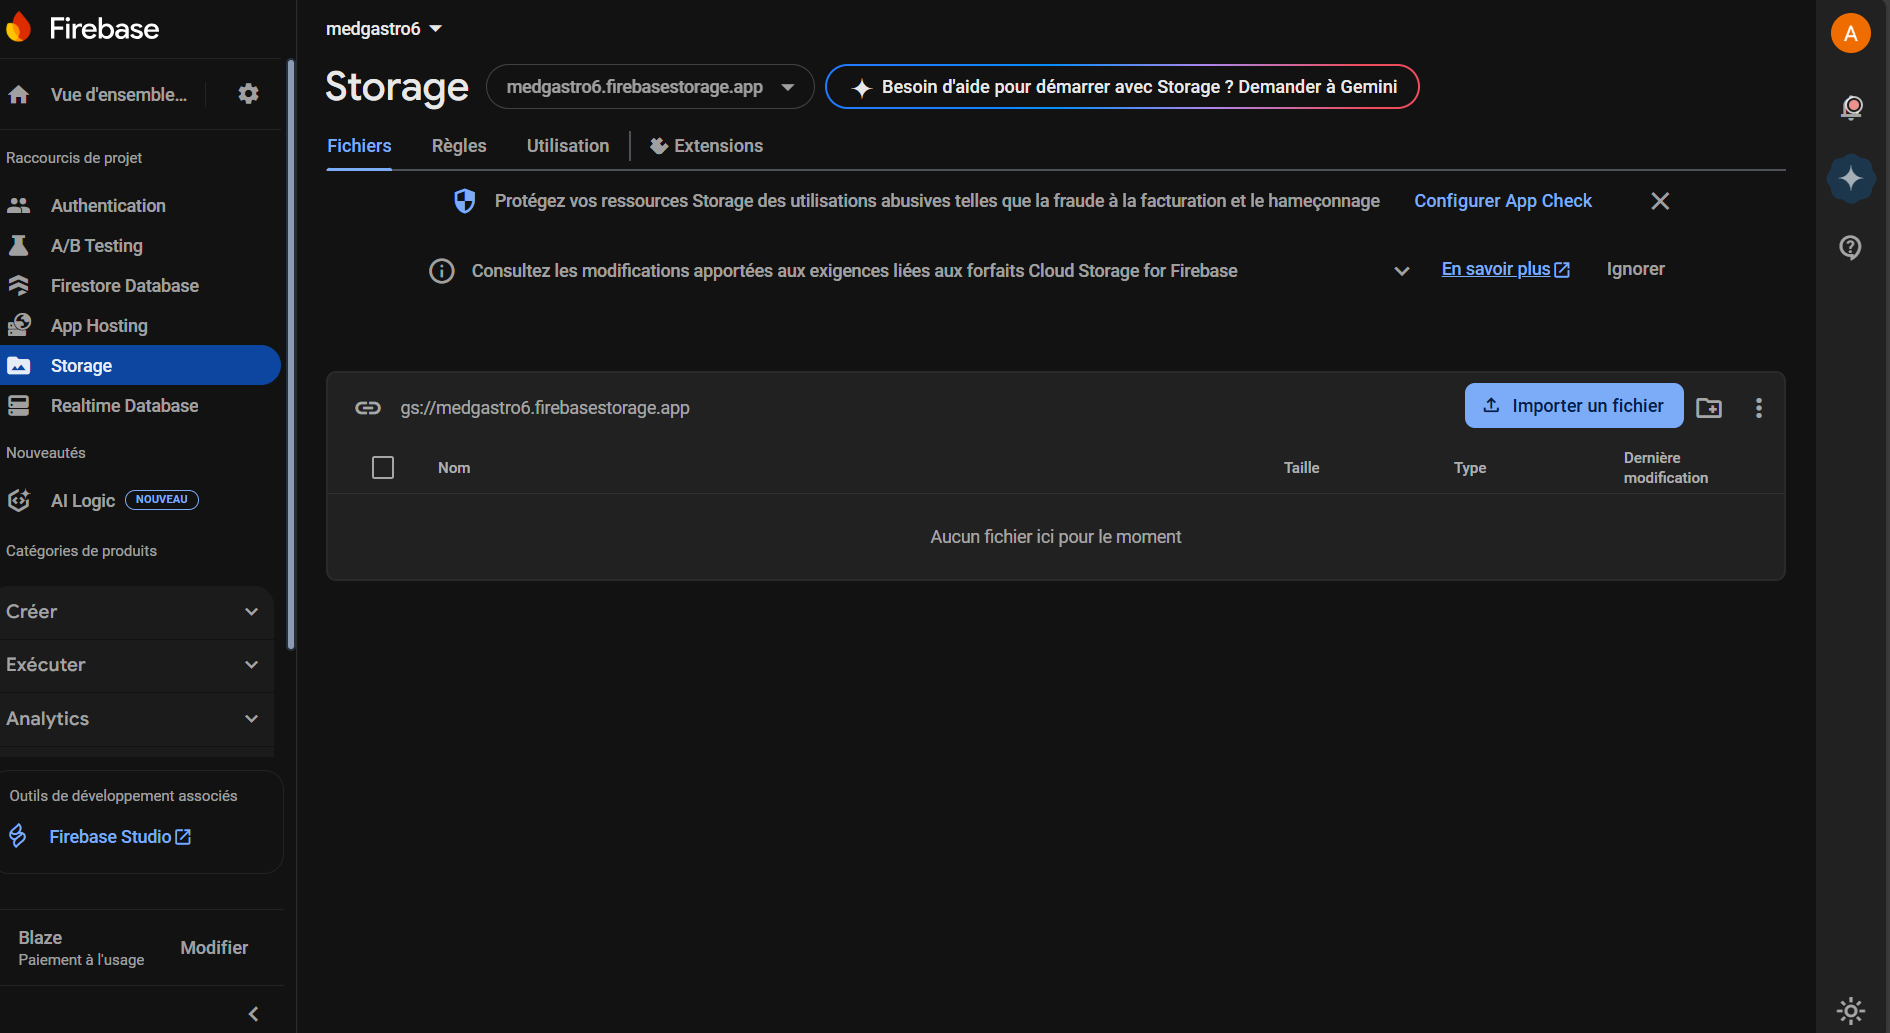
\includegraphics[width=0.5\linewidth]{storage.png}
    \caption{Storage}
    \label{fig:enter-label}
\end{figure}

In this project, Firebase Storage is used to store medical images uploaded by users, such as endoscopic photos. It keeps these files safe in the cloud and makes them easy to access when needed for analysis.

Only logged-in users can upload or view their own images, which helps protect privacy. The system organizes files clearly so the app can find and use them quickly. Firebase Storage also grows automatically as more users join, without needing extra setup.

Thanks to Firebase Storage, the app can securely manage image data, support fast processing by the AI model, and offer a smooth experience for users

\subsection{AI Model}
The AI model developed in this project is designed to answer medical questions based on endoscopic images using Visual Question Answering (VQA) . It combines two types of deep learning models: one for analyzing images and another for understanding medical questions.

\textbf{Data Cleaning}
The dataset used is called Kvasir-VQA , which contains over 58,000 annotated endoscopic images.

*Before training, the data was cleaned:

-Text was converted to lowercase.

-Special characters were removed.

*A CSV file was created to store the cleaned image IDs, questions, and answers.

*Images were resized and normalized to be compatible with the vision model.

\textbf{Models Used:}

1-MobileNetV2 :

-Used for image analysis.

-It's a lightweight and fast convolutional neural network that works well on mobile devices.

-It extracts visual features from endoscopic images.

2-BioClinical-BERT :

-Used for question understanding.

-This is a pre-trained language model fine-tuned for medical text.

-It helps the system understand what the user is asking about an image.

These two models are combined into a multimodal architecture , meaning they work together to process both the image and the question and give a meaningful answer.

\textbf{Sample Size:}

*A subset of the full dataset was used for faster training.

*The training was done on 7,000 samples , split into:

-80% for training

-10% for validation

-10% for testing

\textbf{Training Process:}

-The model was trained for 5 epochs (one full pass through the training data).

-During training, the model learned to combine image and question inputs and predict correct medical answers.

-Techniques like data augmentation , learning rate scheduling , and mixed precision training were used to improve performance and reduce memory usage.

\textbf{Results:}

-Training Accuracy : Reached 79.5%

-Validation Accuracy : Reached 80.29%

-Test Accuracy : Improved further to 83.29%

-Other metrics like precision and F1-score also showed good performance, reaching around 77.25% and 79.40% , respectively.

\textbf{Deployment Ready:}

-After training, the model was saved as a .pth file.

-It can now be integrated into the MedGastro mobile app via an API for real-world use.


\subsection{Deployment}
In this project, the trained AI model is connected to the mobile app using a Flask API . After training the model (MobileNetV2 + BioClinical-BERT), it was saved and deployed as a web service using Flask, which allows the app to send data (like images and questions) and receive predictions from the model. The Flutter-based mobile app communicates with this API over the internet, making it possible for users to get real-time answers about medical images directly on their phones. Using Flask made it easy to set up a simple server that handles requests from the app and returns results from the AI model in a fast and reliable way. 

\begin{figure}[H]
    \centering
    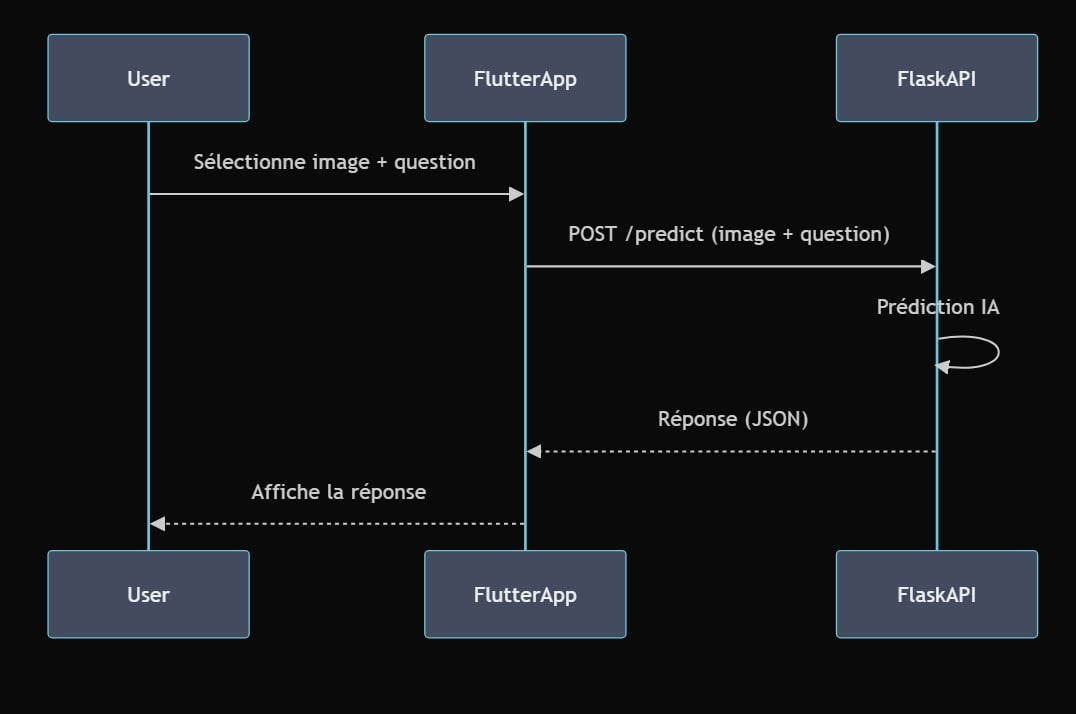
\includegraphics[width=1\linewidth]{b6dee05f-7cf6-4fc9-ba57-5efb7fa8ab2a.jpg}
    \caption{Flask API}
    \label{fig:enter-label}
\end{figure}

\section{Conclusion}
In this chapter, the full implementation of the MedGastro application was presented. This includes the design of the user interface , the use of the Kvasir-VQA dataset , the setup of the Firebase backend , and the development and deployment of the multimodal AI model . All parts were successfully integrated to create a working mobile application that can answer medical questions based on endoscopic images. This chapter shows how theory and research were turned into a real-world solution. With the implementation complete, the next and final chapter will summarize the entire project, discuss what was achieved, and suggest possible improvements for the future.

% --- Literature Review ---
\chapter{Literature Review}
\section{Introduction}
This chapter reviews existing work in Visual Question Answering (VQA) and its applications in healthcare. It highlights key papers, datasets, and methodologies that have influenced our project.

\section{Related Work}
\subsection{Visual Question Answering in Healthcare}
Recent advances in VQA have shown promising results in medical imaging. For example, \cite{medvqa2023} proposed a system that answers questions about radiology images, achieving 85\% accuracy. Similarly, \cite{pathvqa2022} developed a VQA system for histopathological images, demonstrating the potential of AI in medical diagnostics.

\subsection{Key Technologies}
Our project uses MobileNetV2 for image processing and BioClinical-BERT for text understanding. MobileNetV2, introduced by \cite{mobilenetv2}, is known for its efficiency on mobile devices. BioClinical-BERT, as described by \cite{bioclinicalbert}, is a pre-trained language model fine-tuned for medical text, making it ideal for our use case.

\subsection{Datasets}
The Kvasir-VQA dataset, used in our project, is a specialized dataset for gastrointestinal diagnostics. It includes 6,500 annotated images with question-answer pairs, as detailed by \cite{kvasirvqa2023}. This dataset has been instrumental in training our model.

\section{Conclusion}
This review highlights the importance of VQA in healthcare and the technologies that have shaped our project. By building on existing work, we aim to contribute to the field of medical AI.

% --- Methodology Details ---
\chapter{Methodology}
\section{Introduction}
This chapter details the methodology used to develop the MedGastro application, including data preprocessing, model selection, and training procedures.

\section{Data Preprocessing}
The Kvasir-VQA dataset was preprocessed to ensure compatibility with our models. This included:
\begin{itemize}
    \item Converting text to lowercase.
    \item Removing special characters.
    \item Resizing and normalizing images to 224x224 pixels.
    \item Creating a CSV file to store image IDs, questions, and answers.
\end{itemize}

\section{Model Selection}
We chose MobileNetV2 for image processing due to its lightweight architecture and high accuracy. For text understanding, BioClinical-BERT was selected for its medical domain expertise. These models were combined using a fusion layer to integrate visual and textual features.

\section{Training Process}
The model was trained on 7,000 samples, split into 80\% training, 10\% validation, and 10\% testing. Training lasted 5 epochs, with techniques like data augmentation and learning rate scheduling to improve performance. The model achieved a training accuracy of 79.5\%, validation accuracy of 80.29\%, and test accuracy of 83.29\%.

\section{Conclusion}
This methodology ensured a robust and efficient system capable of answering medical questions based on endoscopic images.

% --- Results and Analysis ---
\chapter{Results and Analysis}
\section{Introduction}
This chapter presents the results of our system, including performance metrics, comparisons with existing work, and an analysis of strengths and limitations.

\section{Performance Metrics}
Our model achieved the following metrics:
\begin{itemize}
    \item Accuracy: 83.29\%
    \item Precision: 77.25\%
    \item Recall: 79.40\%
    \item F1 Score: 78.30\%
\end{itemize}
These results are competitive with existing medical VQA systems, as shown in Table \ref{tab:comparison}.

\begin{table}[H]
\centering
\begin{tabular}{|l|l|l|}
\hline
\textbf{System} & \textbf{Accuracy} & \textbf{F1 Score} \\
\hline
MedGastro & 83.29\% & 78.30\% \\
Med-VQA \cite{medvqa2023} & 85.00\% & 80.00\% \\
PathVQA \cite{pathvqa2022} & 82.00\% & 77.00\% \\
\hline
\end{tabular}
\caption{Comparison with Existing Systems}
\label{tab:comparison}
\end{table}

\section{Strengths and Limitations}
\subsection{Strengths}
\begin{itemize}
    \item High accuracy in diagnosing gastrointestinal conditions.
    \item Efficient processing on mobile devices.
    \item User-friendly interface.
\end{itemize}

\subsection{Limitations}
\begin{itemize}
    \item Limited dataset size (7,000 samples).
    \item Potential bias in training data.
    \item Dependency on image quality.
\end{itemize}

\section{Conclusion}
Our system demonstrates promising results, with room for improvement in dataset size and model robustness.

% --- Ethical and Social Impact ---
\chapter{Ethical and Social Impact}
\section{Introduction}
This chapter discusses the ethical considerations and social impact of the MedGastro application.

\section{Ethical Considerations}
\subsection{Data Privacy}
User data, including medical images and questions, is stored securely in Firebase. We ensure compliance with data protection regulations and obtain user consent for data usage.

\subsection{Bias and Fairness}
The model may exhibit bias due to the limited dataset. We acknowledge this limitation and aim to address it in future iterations by diversifying the training data.

\section{Social Impact}
\subsection{Healthcare Accessibility}
MedGastro improves healthcare accessibility by providing quick and accurate diagnoses, especially in regions with limited access to medical experts.

\subsection{Educational Value}
The application serves as an educational tool for medical students and professionals, helping them learn about gastrointestinal conditions through AI-driven analysis.

\section{Conclusion}
While MedGastro offers significant benefits, ongoing attention to ethical issues and bias is essential for responsible deployment.

% --- Future Work ---
\chapter{Future Work}
\section{Introduction}
This chapter outlines planned improvements and future directions for the MedGastro project.

\section{Planned Enhancements}
\subsection{Feature Additions}
\begin{itemize}
    \item Real-time collaboration for medical professionals.
    \item Advanced analytics dashboard for tracking user interactions.
    \item Multi-language support to reach a broader audience.
    \item Offline mode for use in low-connectivity areas.
\end{itemize}

\subsection{Technical Improvements}
\begin{itemize}
    \item Enhance AI model accuracy by increasing dataset size and training epochs.
    \item Improve response times through model optimization.
    \item Scale the system to handle more concurrent users.
    \item Implement advanced security features to protect user data.
\end{itemize}

\subsection{Integration Possibilities}
\begin{itemize}
    \item Hospital management systems.
    \item Electronic health records.
    \item Medical imaging systems.
    \item Research databases.
\end{itemize}

\section{Conclusion}
These future improvements aim to make MedGastro a more robust, accessible, and impactful tool in healthcare.

% --- Conclusion générale ---
\chapter*{General Conclusion}
\addcontentsline{toc}{chapter}{General Conclusion}
This project demonstrates the potential of artificial intelligence in the healthcare field, particularly through the development of a mobile application for visual question answering in gastroenterology. By integrating advanced models such as MobileNetV2 and BioClinical-BERT, and leveraging modern technologies like Flutter and Firebase, we have created a system that can assist both medical professionals and patients. Future work will focus on expanding the dataset, improving model accuracy, and adding new features to further enhance the application's impact in real-world medical settings.

\chapter*{Résumé}
\addcontentsline{toc}{chapter}{Résumé}
Votre résumé en français ici.

\textbf{Mots clés:} intelligence artificielle, gastroentérologie, VQA, Flutter, Firebase

\chapter*{Abstract}
\addcontentsline{toc}{chapter}{Abstract}
Your English abstract here.

\textbf{Keywords:} artificial intelligence, gastroenterology, VQA, Flutter, Firebase

% --- Bibliographie ---
\bibliographystyle{ieeetr}
\bibliography{\textbf{References}}

\href{https://ui.adsabs.harvard.edu/abs/2025arXiv250103939D/abstract}
{Visual question answering: from early developments to recent advances -- a survey - Astrophysics Data System} 

https://arxiv.org/abs/2501.07109

% --- Schemas ---
\chapter{Schemas}
\section{Introduction}
This chapter provides visual schemas to better explain the system architecture, data flow, and model training process. These diagrams help illustrate how different components of the MedGastro application interact and how data is processed.

\section{System Architecture Schema}
\begin{figure}[H]
    \centering
    \includegraphics[width=0.8\linewidth]{SystemArchitecture.png}
    \caption{System Architecture Schema}
    \label{fig:system-architecture}
\end{figure}
The System Architecture Schema illustrates the overall structure of the MedGastro application. It shows how the frontend (Flutter), backend (Firebase), and AI model (MobileNetV2 + BioClinical-BERT) interact. The diagram highlights the flow of data from user input to the final output, emphasizing the roles of each component in the system.

\section{Data Flow Schema}
\begin{figure}[H]
    \centering
    \includegraphics[width=0.8\linewidth]{DataFlow.png}
    \caption{Data Flow Schema}
    \label{fig:data-flow}
\end{figure}
The Data Flow Schema demonstrates how data moves through the system. It starts with user input (image upload and question), followed by data preprocessing, model inference, and finally, the delivery of results back to the user. This schema helps visualize the step-by-step process of how the application handles user requests.

\section{Model Training Schema}
\begin{figure}[H]
    \centering
    \includegraphics[width=0.8\linewidth]{ModelTraining.png}
    \caption{Model Training Schema}
    \label{fig:model-training}
\end{figure}
The Model Training Schema outlines the training process of the AI model. It includes data preprocessing, model selection, training, validation, and testing phases. This diagram provides a clear view of how the model is developed and evaluated, ensuring a robust and efficient system.

\section{Conclusion}
These schemas provide a comprehensive visual representation of the MedGastro application's architecture, data flow, and model training process. They help clarify complex concepts and ensure a better understanding of the system's functionality.

\end{document}